% !Mode:: "TeX:UTF-8"
% Translator: Shenjian Zhao
\chapter{\glsentrytext{AE}}
\label{chap:autoencoders}
\firstgls{AE}是\gls{NN}的一种,经过训练后能尝试将输入复制到输出。
\firstgls{AE}内部有一个隐含层$\Vh$,可以产生\firstgls{code}来表示输入。
该网络可以看作由两部分组成:一个\gls{encoder}函数$ \Vh = f(\Vx)$和一个生成\gls{reconstruction}的\gls{decoder}$\Vr=g(\Vh)$。
\figref{fig:chap14_autoencoder}展示了这种架构。
如果一个\gls{AE}学会简单地设置$g(f(\Vx)) =\Vx$,那么这个\gls{AE}不会很有用。
相反,\gls{AE}应该被设计成不能学会完美地复制。
这通常需要强加一些约束,使\gls{AE}只能近似地复制,并只能复制类似训练数据的输入。
这些约束强制模型划定输入数据不同方面的主次顺序,因此它往往能学习到数据的有用特性。


现代\gls{AE}将\gls{encoder}和\gls{decoder}的思想推广,将其中的确定函数推广为随机映射$p_{\text{encoder}} (\Vh | \Vx)$和$p_{\text{decoder}}(\Vx | \Vh)$。


数十年间,\gls{AE}的想法一直是\gls{NN}历史景象的一部分~\citep{Lecun-these87,Bourlard88,hinton1994amd-small}。
传统上,\gls{AE}被用于\gls{dimensionality_reduction}或特征学习。
近年来,\gls{AE}与隐变量模型理论的联系将\gls{AE}带到了生成建模的前沿,我们将在\chapref{chap:deep_generative_models}看到更多细节。
\gls{AE}可以被看作是\gls{feedforward_network}的一种特殊情况,并且可以使用完全相同的技术进行训练,通常使用\gls{minibatch}\gls{GD}法(基于\gls{back_propagation}计算的梯度)。
不像一般的\gls{feedforward_network},\gls{AE}也可以使用\firstgls{recirculation}训练\citep{Hinton+McClelland-NIPS1987},这是一种基于比较原始输入和\gls{reconstruction}输入激活的学习算法。
相比\gls{back_propagation}算法,\gls{recirculation}算法从生物学上看似更有道理,但很少用于\gls{ML}。

\begin{figure}[!htb]
\ifOpenSource
\centerline{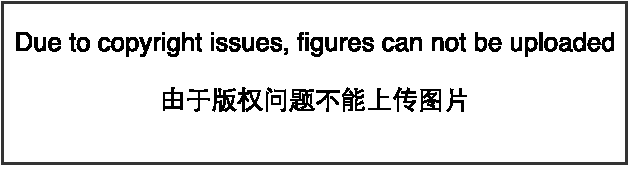
\includegraphics{figure.pdf}}
\else
\centerline{\includegraphics{Chapter14/figures/autoencoder}}
\fi
\caption{TODO}
\label{fig:chap14_autoencoder}
\end{figure}

% -- 493 --

\section{\glsentrytext{undercomplete}\glsentrytext{AE}}
\label{sec:undercomplete_autoencoders}
将输入复制到输出听起来没什么用,但我们通常不关心\gls{decoder}的输出。
相反,我们希望通过训练\gls{AE}对输入进行复制的任务使$\Vh$获得有用的特性。


从\gls{AE}获得有用特征的一种方法是限制$\Vh$的维度比$\Vx$小,这种\gls{code}维度小于输入维度的\gls{AE}称为\firstgls{undercomplete}\gls{AE}。
学习\gls{undercomplete}的\gls{representation}将强制\gls{AE}捕捉训练数据中最显著的特征。


学习过程可以简单地描述为最小化一个\gls{loss_function} 
\begin{align}
L(\Vx, g(f(\Vx)),
\end{align}
其中$L$是一个\gls{loss_function},衡量$g(f(\Vx))$与$\Vx$的不相似性,如\gls{mean_squared_error}。


当\gls{decoder}是线性的且$L$是\gls{mean_squared_error},\gls{undercomplete}的\gls{AE}会学习出与\glssymbol{PCA}相同生成子空间。
在这种情况下,\gls{AE}学到了训练数据的主元子空间(执行复制任务的副效用)。


因此拥有非线性编码函数$f$和非线性\gls{decoder}函数$g$的\gls{AE}能够学习出更强大的\glssymbol{PCA}非线性推广。
不幸的是,如果\gls{encoder}和\gls{decoder}被赋予太大的\gls{capacity},\gls{AE}会执行复制任务而捕捉不到有关数据分布的有用信息。
从理论上说,我们可以想象只有一维\gls{code}的\gls{AE},但具有一个非常强大的非线性\gls{encoder},能够将每个训练数据$\Vx^{(i)}$表示为\gls{code}$~i$。
\gls{decoder}可以学习将这些整数索引映射回特定训练样本的值。
这种特定情形不会在实践中发生,但它清楚地说明,如果\gls{AE}的\gls{capacity}太大,那训练来执行复制任务的\gls{AE}可能无法学习到数据集的任何有用信息。

% -- 494 --

\section{正则\glsentrytext{AE}}
\label{sec:regularized_autoencoders}
\gls{code}维数小于输入维数的\gls{undercomplete}\gls{AE}可以学习数据分布最显著的特征。
我们已经看到,如果这类\gls{AE}被赋予过大的\gls{capacity},它就不能学到任何有用的信息。


如果隐藏层\gls{code}的维数允许与输入相等,或隐藏层\gls{code}维数大于输入的\firstgls{overcomplete}情况下,会发生类似的问题。
在这些情况下,即使是线性\gls{encoder}和线性\gls{decoder}也可以学会将输入复制到输出,而学不到任何有关数据分布的有用信息。


理想情况下,根据要建模的数据分布的复杂性,选择合适的\gls{code}维数和\gls{encoder}、\gls{decoder}
\gls{capacity},就可以成功训练任意架构的\gls{AE}。
正则\gls{AE}提供这样做的可能。
正则\gls{AE}使用的\gls{loss_function}可以鼓励模型学习其它特性(除了将输入复制到输出),而不用限制使用浅层的\gls{encoder}和\gls{decoder}以及小的\gls{code}维数来限制模型的\gls{capacity}。
这些特性包括\gls{sparse}\gls{representation}、\gls{representation}的小导数、以及对噪声或输入缺失的鲁棒性。
即使模型\gls{capacity}大到足够学习一个简单的复制功能,非线性且\gls{overcomplete}的正则\gls{AE}仍然能学到一些与数据分布相关的有用信息。


除了这里所描述的方法(\gls{regularization}\gls{AE}最自然的解释),几乎任何带有隐变量并配有一个\gls{inference}过程(计算给定输入的隐含表示)的\gls{generative_model},都可以看作是\gls{AE}的一种特殊形式。
强调与\gls{AE}联系的两个生成建模方法是\gls{helmholtz_machine}~\citep{Hinton95}的衍生模型,如\gls{VAE}(\secref{sec:variational_autoencoders})和\gls{GSN}(\secref{sec:generative_stochastic_networks})。
这些模型能自然地学习大\gls{capacity}、对输入\gls{overcomplete}的有用编码,而不需要\gls{regularization}。
这些\gls{code}显然是有用的,因为这些模型被训练为近似训练数据的最大概率而不是将输入复制到输出。

% -- 495 --

\subsection{\glsentrytext{sparse}\glsentrytext{AE}}
\label{sec:sparse_autoencoders}
\gls{sparse}\gls{AE}简单地在训练时结合\gls{code}层的\gls{sparse}惩罚$\Omega(\Vh)$和\gls{reconstruction_error}:
\begin{align}
L(\Vx, g(f(\Vx)) + \Omega(\Vh),
\end{align}
其中$g(\Vh)$是\gls{decoder}的输出,通常$\Vh$是\gls{encoder}的输出,即$\Vh = f(\Vx)$。


\gls{sparse}\gls{AE}通常用于学习特征,以便用于其他任务如分类。
\gls{sparse}\gls{regularization}的\gls{AE}必须反映训练数据集的独特统计特征,而不是简单地充当恒等函数。
以这种方式训练,执行附带\gls{sparse}罚的复制任务可以得到能学习有用特征的模型。


我们可以简单地将惩罚项$\Omega(\Vh)$视为加到\gls{feedforward_network}的正则项,这个\gls{feedforward_network}的主要任务是将输入复制到输出(\gls{unsupervised_learning}的目标),并尽可能地根据这些\gls{sparse}特征执行一些\gls{supervised_learning}任务(根据\gls{supervised_learning}的目标)。
不像其它正则项如\gls{weight_decay},这个\gls{regularization}没有直观的贝叶斯解释。
如\secref{sec:maximum_a_posteriori_map_estimation}描述,\gls{weight_decay}和其他正则惩罚可以被解释为一个\glssymbol{MAP}近似贝叶斯\gls{inference},\gls{regularization}的惩罚对应于模型参数的先验概率分布。
这种观点认为,\gls{regularization}的最大似然对应最大化$p(\Vtheta | \Vx)$, 相当于最大化$\log p(\Vx ~|~ \Vtheta) + \log p(\Vtheta)$。 $\log p(\Vx | \Vtheta)$即通常的数据似然项,参数的对数先验项$\log p(\Vtheta)$则包含了对$\Vtheta$特定值的偏好。
这种观点在\secref{sec:bayesian_statistics}有所描述。
正则\gls{AE}不适用这样的解释是因为正则项取决于数据,因此根据定义上(从文字的正式意义)来说,它不是一个先验。
我们仍可以认为这些正则项隐式地表达了对函数的偏好。

% -- 496 --

我们可以认为整个\gls{sparse}\gls{AE}框架是对带有隐变量的\gls{generative_model}的近似最大似然训练,而不将\gls{sparse}惩罚视为复制任务的\gls{regularization}。
假如我们有一个带有可见变量$\Vx$和隐变量$\Vh$的模型,且具有明确的联合分布$p_{\text{model}}(\Vx,\Vh)=p_{\text{model}}(\Vh)p_{\text{model}} (\Vx ~|~ \Vh)$。
<BAD>我们将$p_{\text{model}}(\Vh)$视为模型关于隐变量的先验分布,表示模型看到$\Vx$的信念先验。
这与我们之前使用``先验''的方式不同,之前指分布$p(\Vtheta)$在我们看到数据前就对模型参数的先验进行编码。
对数似然函数可分解为
\begin{align}
\log p_{\text{model}}(\Vx)=\log \sum_{\Vh} p_{\text{model}}(\Vh, \Vx) .
\end{align}
我们可以认为\gls{AE}使用一个高似然值$\Vh$的点估计来近似这个总和。
这类似于\gls{sparse_coding}\gls{generative_model}(\secref{sec:sparse_coding}),但$\Vh$是参数\gls{encoder}的输出,而不是从优化结果推断出的最可能的$\Vh$。
从这个角度看,我们根据这个选择的$\Vh$,最大化如下
\begin{align}
\log p_{\text{model}}(\Vh, \Vx)=\log p_{\text{model}}(\Vh) + \log p_{\text{model}}(\Vx ~|~ \Vh) .
\end{align}
$\log p_{\text{model}}(\Vh) $ 项能被\gls{sparse}诱导。
如\ENNAME{Laplace}先验,
\begin{align}
p_{\text{model}}(h_i) = \frac{\lambda}{2} e^{-\lambda | h_i |},
\end{align}
对应于绝对值\gls{sparse}惩罚。
将对数先验表示为绝对值惩罚,我们得到
\begin{align}
\Omega(\Vh) &= \lambda \sum_{i} | h_i  |,\\ 
-\log p_{\text{model}}(\Vh) &= 
\sum_i (\lambda | h_i | - \log \frac{\lambda}{2}) = \Omega(\Vh) + \text{const},
\end{align}
这里的常数项只跟$\lambda$有关。
通常我们将$\lambda$视为超参数,因此可以丢弃不影响参数学习的常数项。
其它如\ENNAME{Student-t}先验也能诱导\gls{sparse}性。
从\gls{sparse}性导致$p_{\text{model}}(\Vh)$学习成近似最大似然的结果看,\gls{sparse}惩罚完全不是一个正则项。
这仅仅影响模型关于隐变量的分布。
这个观点提供了训练\gls{AE}的另一个动机:这是近似训练\gls{generative_model}的一种途径。
这也给出了为什么\gls{AE}学到的特征是有用的另一个解释:它们描述的隐变量可以解释输入。

% -- 497 --

\gls{sparse}\gls{AE}的早期工作~\citep{ranzato-07-small,ranzato-08-small}探讨了各种形式的\gls{sparse}性,并提出了\gls{sparse}惩罚和$\log  Z$项(将最大似然应用到无向概率模型$p(\Vx)=\frac{1}{Z}\tilde{p}(\Vx)$时产生)之间的联系。
这个想法是最小化$\log Z$防止概率模型处处具有高概率,同理强制\gls{sparse}可以防止\gls{AE}处处具有低的\gls{reconstruction_error} 。
这种情况下,这种联系是对通用机制的直观理解而不是数学上的对应。
在数学上更容易解释\gls{sparse}惩罚对应于有向模型$p_{\text{model}}(\Vh)p_{\text{model}}(\Vx ~|~ \Vh) $中的$\log p_{\text{model}}(\Vh)$。


\citet{Glorot+al-ICML-2011-small}提出了一种在\gls{sparse}(和\gls{denoising})\gls{AE}的$\Vh$中实现\emph{真正为零}的方式。
该想法是使用\gls{ReLU}来产生\gls{code}层。
基于将\gls{representation}真正推向零(如绝对值惩罚)的先验,可以间接控制\gls{representation}中零的平均数量。



\subsection{\glsentrytext{DAE}}
\label{sec:sub_denoising_autoencoders}
除了向\gls{cost_function}增加一个惩罚项,我们也可以改变\gls{reconstruction_error}项得到一个能学到有用信息的\gls{AE}。


传统的\gls{AE}最小化以下目标
\begin{align}
L(\Vx, g(f(\Vx)),
\end{align}
其中$L$是一个\gls{loss_function},衡量$g(f(\Vx))$与$\Vx$的不相似性,如它们不相似度的$L^2$范数。
如果模型被赋予足够的\gls{capacity},$L$仅仅鼓励$g \circ  f$学成一个恒等函数。


相反,\firstall{DAE}最小化 
\begin{align}
L(\Vx, g(f(\tilde \Vx)),
\end{align}
其中 $\tilde \Vx$是被某种噪声损坏的$\Vx$的副本。
因此\gls{DAE}必须撤消这些损坏,而不是简单地复制输入。

\citet{Alain+Bengio-ICLR2013-small}和\citet{Bengio-et-al-NIPS2013-small}指出\gls{denoising}训练过程强制$f$和$g$隐式地学习$p_{\text{data}} (\Vx)$的结构。
因此\gls{DAE}也是一个通过最小化\gls{reconstruction_error}来获取有用特性的例子。
这也是将\gls{overcomplete}、高\gls{capacity}的模型用作\gls{AE}的一个例子——只要小心防止这些模型仅仅学习一个恒等函数。
\gls{DAE}将在\secref{sec:denoising_autoencoders}给出更多细节。

% -- 498 --

\subsection{惩罚导数作为正则}
\label{sec:regularizing_by_penalizing_derivatives}
另一正则化\gls{AE}的策略是使用一个类似\gls{sparse}\gls{AE}中的惩罚项$\Omega$,
\begin{align}
L(\Vx, g(f(\Vx)) + \Omega(\Vh, \Vx),
\end{align}
但$\Omega$的形式不同:
\begin{align}
\Omega(\Vh, \Vx) = \lambda \sum_i \| \nabla_{\Vx}h_i \|^2.
\end{align}


这迫使模型学习一个在$\Vx$变化小时目标也没有太大变化的函数。
因为这个惩罚只对训练数据适用,它迫使\gls{AE}学习可以反映训练数据分布信息的特征。


这样\gls{regularization}的\gls{AE}被称为\firstall{CAE}。
这种方法与\gls{DAE}、\gls{manifold_learning}和概率模型存在一定理论联系。
\gls{CAE}在\secref{sec:contractive_autoencoders}有更详细的描述。


\section{表示能力、层的大小和深度}
\label{sec:representational_power_layer_size_and_depth}
\gls{AE}通常只有单层的\gls{encoder}和\gls{decoder},但这不是必然的。
实际上深度\gls{encoder}和\gls{decoder}能提供更多优势。


回忆\secref{sec:universal_approximation_properties_and_depth},其中提到加深\gls{feedforward_network}有很多优势。
这些优势也同样适用于\gls{AE},因为它也属于\gls{feedforward_network}。
此外,\gls{encoder}和\gls{decoder}自身都是一个\gls{feedforward_network},因此这两个部分也能各自从深度中获得好处。


普遍逼近定理保证至少有一层隐含层且\gls{hidden_unit}足够多的\gls{feedforward_neural_network}能以任意精度近似任意函数(在很大范围里),这是非平凡深度的一个主要优点。
这意味着单层隐藏层的\gls{AE}在数据范围能表示任意接近数据的恒等函数。
但是,从输入到\gls{code}的映射是浅层的。
这意味这我们不能任意添加约束,比如约束\gls{code}\gls{sparse}。
\gls{encoder}至少包含一层额外隐藏层的深度\gls{AE}能够在给定足够多\gls{hidden_unit}的情况,以任意精度近似任何从输入到\gls{code}的映射。

% -- 499 --

深度可以指数减少表示某些函数的计算成本。
深度也能指数减少学习一些函数所需的训练数据量。
可以参考\secref{sec:universal_approximation_properties_and_depth}巩固深度在\gls{feedforward_network}中的优势。


实验中,深度\gls{AE}能比相应的浅层或线性\gls{AE}产生更好的压缩效率\citep{Hinton-Science2006}。

训练深度\gls{AE}的普遍的策略是训练一堆浅层的\gls{AE}来贪心地预训练相应的深度架构。
所以我们经常会遇到浅层\gls{AE},即使最终目标是训练深度\gls{AE}。


\section{随机\glsentrytext{encoder}和\glsentrytext{decoder}}
\label{sec:stochastic_encoders_and_decoders}
\gls{AE}仅仅是一个\gls{feedforward_network},可以使用与传统的\gls{feedforward_network}同样的\gls{loss_function}和输出单元。


如\secref{sec:other_output_types}中描述,设计\gls{feedforward_network}的输出单元和\gls{loss_function}普遍策略是定义一个输出分布$p(\Vy ~|~ \Vx) $并最小化负的对数似然$-\log p(\Vy ~|~ \Vx)$。
在这种情况下,$\Vy$是关于目标的向量(如类标)。


在\gls{AE}中,$\Vx$既是输入也是目标。
然而,我们仍然可以使用与之前相同的架构。
给定一个隐藏层\gls{code}$\Vh$,我们可以认为\gls{decoder}提供了一个条件分布$p_{\text{model}}(\Vx ~|~ \Vh)$. 
接着我们根据最小化$-\log p_{\text{decoder}}(\Vx ~|~ \Vh)$来训练\gls{AE}。
\gls{loss_function}的具体形式视$p_{\text{decoder}}$的形式而定。
就传统的\gls{feedforward_network}来说,我们通常使用线性输出单元来参数化高斯分布的均值(如果$\Vx$是实的)。
在这种情况下,负对数似然就对应\gls{mean_squared_error}\gls{criterion}。
类似地,二值$\Vx$对应参数由\ENNAME{sigmoid}单元确定的\gls{bernoulli_distribution},离散的$\Vx$对应\ENNAME{softmax}分布等等。
为了便于计算概率分布,通常认为输出变量与给定$\Vh$是条件独立的,但一些技术(如混合密度输出)可以解决输出相关的建模。

% -- 500 --

为了更彻底地区别之前看到的\gls{feedforward_network},我们也可以将\textbf{编码函数}(encoding function)~$f(\Vx)$的概念推广为\textbf{编码分布}(encoding distribution)~$ p_{\text{encoder}}(\Vh | \Vx)$, 如\figref{fig:chap14_stochastic-autoencoder}中所示。

\begin{figure}[!htb]
\ifOpenSource
\centerline{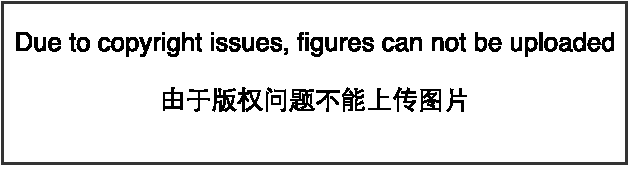
\includegraphics{figure.pdf}}
\else
\centerline{\includegraphics{Chapter14/figures/stochastic-autoencoder}}
\fi
\caption{TODO}
\label{fig:chap14_stochastic-autoencoder}
\end{figure}

任何隐变量模型$p_{\text{model}}(\Vh, \Vx)$定义了一个随机\gls{encoder}
\begin{align}
p_{\text{encoder}}(\Vh ~|~ \Vx) = p_{\text{model}}(\Vh~|~\Vx)
\end{align}
以及一个随机\gls{decoder}
\begin{align}
p_{\text{decoder}}(\Vx ~|~ \Vh) = p_{\text{model}}(\Vx~|~\Vh).
\end{align}
一般情况下,\gls{encoder}和\gls{decoder}的分布没有必要与一个唯一的联合分布$p_{\text{model}}(\Vx, \Vh)$的条件分布相容。
\citet{Alain-et-al-arxiv2015}指出将\gls{encoder}和\gls{decoder}作为\gls{DAE}来训练能使它们渐近地相容(有足够的\gls{capacity}和样本)。



\section{\glsentrytext{DAE}}
\label{sec:denoising_autoencoders}
\firstall{DAE}是一类接受损坏数据作为输入,并训练来预测原始未被损坏数据作为输出的\gls{AE}。

% -- 501 --

\glssymbol{DAE}的训练过程如\figref{fig:chap14_DAE}中所示。
我们引入一个损坏过程$C(\tilde{\RVx} ~|~ \RVx)$,这个条件分布代表给定数据样本$\RVx$产生损坏样本$\tilde \RVx$的概率。
\gls{AE}则根据以下过程,从训练数据对$(\Vx, \tilde \Vx)$中学习\textbf{重构分布}(reconstruction distribution)~$p_{\text{reconstruct}} (\RVx ~|~ \tilde \RVx)$:
\begin{enumerate}
\item 从训练数据中采一个训练样本$\Vx$。
\item 从$C(\tilde{\RVx} ~|~ \RVx=\Vx)$采一个损坏样本$\tilde \Vx$。
\item 将$(\Vx, \tilde \Vx)$作为训练样本来估计\gls{AE}的\gls{reconstruction}分布 
$p_{\text{reconstruct}} (\Vx ~|~ \tilde \Vx) = p_{\text{decoder}}(\Vx ~|~\Vh)$,其中$\Vh$是\gls{encoder}$f(\tilde \Vx)$的输出,$p_{\text{decoder}}$根据解码函数$g(\Vh)$定义。
\end{enumerate}
通常我们可以简单地对负对数似然$-\log p_{\text{decoder}} (\Vx | \Vh)$进行基于梯度法(如\gls{minibatch}\gls{GD})的近似最小化。
只要\gls{encoder}是确定性的,\gls{DAE}就是一个\gls{feedforward_network},并且可以使用与其他\gls{feedforward_network}完全相同的方式进行训练。

\begin{figure}[!htb]
\ifOpenSource
\centerline{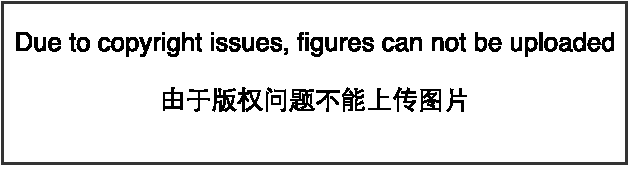
\includegraphics{figure.pdf}}
\else
\centerline{\includegraphics{Chapter14/figures/DAE}}
\fi
\caption{TODO}
\label{fig:chap14_DAE}
\end{figure}

因此我们可以认为\glssymbol{DAE}是在以下期望下进行\gls{SGD}:
\begin{align}
   - \SetE_{\RVx \sim \hat{p}_{\text{data}}(\RVx)} \SetE_{\tilde{\RVx} \sim C(\tilde{\RVx}\mid\Vx)} \log p_{\text{decoder}}(\Vx \mid \Vh = f(\tilde{\Vx})),
\end{align}
其中$\hat{p}_{\text{data}}(\Vx)$是训练数据的分布。

% -- 502 --

\subsection{\glsentrytext{score}估计}
\label{sec:estimating_the_score}
\gls{score_matching}\citep{Hyvarinen-2005}是最大似然的代替。
它提供了概率分布的一致估计,鼓励模型在各个数据点$\Vx$上获得与数据分布相同的\firstgls{score}。
在这种情况下,\gls{score}是一个特定的梯度场:
\begin{align}
 \nabla_{\Vx} \log p(\Vx) .
\end{align}

将在\secref{sec:score_matching_and_ratio_matching}中更详细的讨论\gls{score_matching}。
对于现在讨论的\gls{AE},理解学习$\log p_{\text{data}}$的梯度场是学习$p_{\text{data}}$结构的一种方式就足够了。


\glssymbol{DAE}的训练\gls{criterion})(条件高斯$p(\Vx \mid \Vh)$)能让\gls{AE}学到能估计数据分布得分的向量场$(g(f(\Vx))-\Vx)$ ,这是\glssymbol{DAE}的一个重要特性。
具体如\figref{fig:chap14_denoising_task}所示。

\begin{figure}[!htb]
\ifOpenSource
\centerline{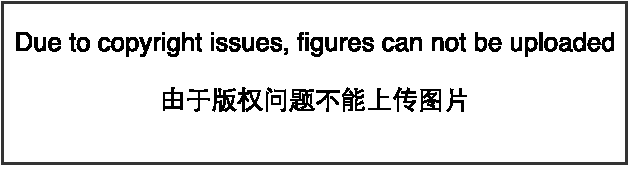
\includegraphics{figure.pdf}}
\else
\centerline{\includegraphics{Chapter14/figures/denoising_task}}
\fi
\caption{TODO}
\label{fig:chap14_denoising_task}
\end{figure}

\gls{denoising}地训练一类采用高斯噪声和\gls{mean_squared_error}作为\gls{reconstruction_error}的特定\gls{DAE}(sigmoid\gls{hidden_unit}, 线性\gls{reconstruction}单元),与训练一类特定的被称为\glssymbol{RBM}的无向概率模型是等价的\citep{Vincent-NC-2011-small}。
这类模型将在\secref{sec:gaussian_bernoulli_rbms}给出更详细的介绍;对于现在的讨论,我们只需知道这个模型能显式的给出$p_{\text{model}}(\Vx; \Vtheta)$。
当\glssymbol{RBM}使用\firstgls{denoising_score_matching}~\citep{Kingma+LeCun-2010-small}训练时,它的学习算法与训练对应的\gls{DAE}是等价的。
在一个确定的噪声水平下,\gls{regularization}的\gls{score_matching}不是一致估计量;相反它会恢复分布的一个模糊版本。
然而,当噪声水平趋向于0且训练样本数趋向与无穷时,一致性就会恢复。
将会在\secref{sec:denoising_score_matching}更详细地讨论\gls{denoising_score_matching}。


\gls{AE}和\glssymbol{RBM}还存在其它联系。
\gls{score_matching}应用于\glssymbol{RBM}后,其\gls{cost_function}将等价于\gls{reconstruction_error}结合类似\glssymbol{CAE}惩罚的正则项 \citep{Swersky-ICML2011}。
\citet{Bengio+Delalleau-2009}指出\gls{AE}的\gls{gradient}是对\glssymbol{RBM}\gls{contrastive_divergence}训练的近似。


对于连续的$\Vx$,高斯损坏和\gls{reconstruction}分布的\gls{denoising}\gls{criterion}得到的\gls{score}估计适用于一般\gls{encoder}和\gls{decoder}的参数化\citep{Alain+Bengio-ICLR2013-small}。
这意味着一个使用平方误差\gls{criterion}
\begin{align}
 \| g(f(\tilde \Vx)) - \Vx \|^2
\end{align}
和噪声方差为$\sigma^2 $的损坏
\begin{align}
 C(\tilde x = \tilde \Vx | \Vx) = N(\tilde \Vx; \mu=\Vx, \Sigma = \sigma^2 I)
\end{align}
的通用\gls{encoder}-\gls{decoder}架构可以用来训练估计\gls{score}。
\figref{fig:chap14_vector_field_color}展示其中的工作原理。

\begin{figure}[!htb]
\ifOpenSource
\centerline{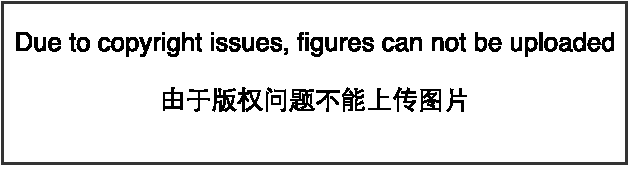
\includegraphics{figure.pdf}}
\else
\centerline{\includegraphics[width=0.8\textwidth]{Chapter14/figures/vector_field_color}}
\fi
\caption{TODO}
\label{fig:chap14_vector_field_color}
\end{figure}

一般情况下,不能保证\gls{reconstruction}函数$g(f(\Vx))$减去输入$\Vx$后对应于某个函数的\gls{gradient},更不用说\gls{score} 。
这是早期工作~\citep{Vincent-NC-2011-small}专用于特定参数化的原因(其中$g(f(\Vx)) - \Vx$能通过另一个函数的导数获得)。
\citet{Kamyshanska+Memisevic-2015}通过标识一类特殊的浅层\gls{AE}家族,使$g(f(\Vx)) - \Vx$对应于这个家族所有成员的一个\gls{score},以此推广\citet{Vincent-NC-2011-small}的结果。

% -- 504 --

目前为止我们所讨论的仅限于\gls{DAE}如何学习表示一个概率分布。
更一般的,我们可能希望使用\gls{AE}作为\gls{generative_model},并从该分布中进行采样。
这将在\secref{sec:drawing_samples_from_autoencoders}中讨论。

% -- 505 --

\subsection{历史观点}
\label{sec:historical_perspective_chap14}
采用\glssymbol{MLP}\gls{denoising}的想法可以追溯到\cite{Lecun-these87}和\citet{Gallinari87}的工作。
\citet{Behnke-2001}也曾使用\gls{recurrent_network}对图像去噪。
在某种意义上,\gls{DAE}仅仅是被训练\gls{denoising}的\glssymbol{MLP}。
然而,``\gls{DAE}''的命名指的不仅仅是学习\gls{denoising},而且可以学到一个好的内部\gls{representation}(作为学习\gls{denoising}的副效用)。
这个想法提出较晚\citep{VincentPLarochelleH2008-small,Vincent-JMLR-2010-small}。
学习到的\gls{representation}可以被用来预训练更深的\gls{unsupervised}网络或\gls{supervised}网络。
与\gls{sparse}\gls{AE}、\gls{sparse_coding}、\gls{CAE}等\gls{regularization}的\gls{AE}类似, \glssymbol{DAE}的动机是允许使用一个\gls{capacity}非常大的\gls{encoder},同时防止在\gls{encoder}和\gls{decoder}学习一个毫无用处的恒等函数 。


在引入现代\glssymbol{DAE}之前,\citet{Inayoshi-and-Kurita-2005}探讨了与一些相同的方法和相同的目标。
他们的做法在有\gls{supervised}目标的情况下最小化\gls{reconstruction_error} ,并在监督\glssymbol{MLP}的隐藏层注入噪声,通过引入\gls{reconstruction_error}和注入噪声提升泛化能力。
然而,他们的方法基于线性\gls{encoder},因此无法学习到现代\glssymbol{DAE}能学习的强大函数族。



\section{使用\glsentrytext{AE}学习\glsentrytext{manifold}}
\label{sec:learning_manifolds_with_autoencoders}

如\secref{sec:manifold_learning}描述,\gls{AE}跟其它很多\gls{ML}算法一样,也应用了将数据集中在一个低维\gls{manifold}或者一小组这样的\gls{manifold}的思想。
其中一些\gls{ML}算法仅能学习到在\gls{manifold}上表现良好但给定不在\gls{manifold}上的输入会导致异常的函数。
\gls{AE}进一步借此想法,旨在学习\gls{manifold}的结构。


要了解\gls{AE}如何做到这一点,我们必须介绍\gls{manifold}的一些重要特性。


\gls{manifold}的一个重要特征是\firstgls{tangent_plane}的集合。
$d$维\gls{manifold}上的一点$\Vx$,\gls{tangent_plane}由能张成\gls{manifold}上允许变动的局部方向的$d$维基向量给出。
如\figref{fig:chap14_tangent_plane_color}所示,这些局部方向说明了我们能如何微小地改变$\Vx$但一直处于\gls{manifold}上。

\begin{figure}[!htb]
\ifOpenSource
\centerline{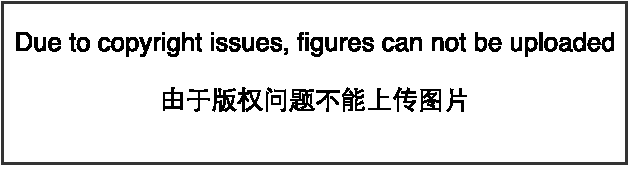
\includegraphics{figure.pdf}}
\else
\centerline{\includegraphics{Chapter14/figures/tangent_plane_color}}
\fi
\caption{TODO}
\label{fig:chap14_tangent_plane_color}
\end{figure}

% -- 506 --

所有\gls{AE}的训练过程涉及两种推动力的折衷:
\begin{enumerate}
 \item 学习训练样本$\Vx$的\gls{representation}$\Vh$使得$\Vx$能通过\gls{decoder}近似地从$\Vh$中恢复。
$\Vx$是从训练数据挑出的事实是关键的,因为这意味着在\gls{AE}不需要成功\gls{reconstruction}不属于数据生成分布下的输入。
 \item 满足约束或正则惩罚。
这可以是限制\gls{AE}\gls{capacity}的架构约束,也可以是加入到\gls{reconstruction}代价的一个正则项。
这些技术一般倾向那些对输入较不敏感的解。
\end{enumerate}

% -- 507 --

显然,单一的推动力是无用的——从它本身将输入复制到输出是无用的,同样忽略输入也是没用的。
相反,两种推动力结合是有用的,因为它们迫使隐藏的表示能捕获有关数据分布结构的信息。
重要的原则是,\gls{AE}必须有能力表示\emph{\gls{reconstruction}训练实例所需的变化}。
如果该数据生成分布集中靠近一个低维\gls{manifold},\gls{AE}能隐式产生捕捉这个\gls{manifold}局部坐标系的表示:仅在$\Vx$周围关于\gls{manifold}的相切变化需要对应于$\Vh=f(\Vx)$中的变化。
因此,\gls{encoder}学习从输入空间$\Vx$到表示空间的映射,映射仅对沿着\gls{manifold}方向的变化敏感,并且对\gls{manifold}正交方向的变化不敏感。


\figref{fig:chap14_1d_autoencoder_color}中一维的例子,说明使\gls{reconstruction}函数对数据点周围的扰动输入不敏感,我们可以让\gls{AE}恢复\gls{manifold}的结构。

\begin{figure}[!htb]
\ifOpenSource
\centerline{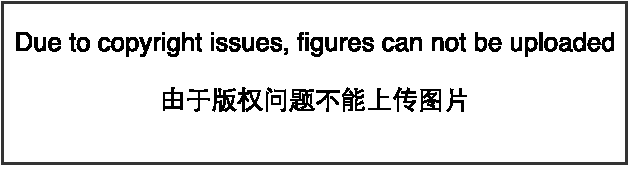
\includegraphics{figure.pdf}}
\else
\centerline{\includegraphics{Chapter14/figures/1d_autoencoder_color}}
\fi
\caption{TODO}
\label{fig:chap14_1d_autoencoder_color}
\end{figure}

% -- 508 --

对比其他的方法是有用且受启发的,可以了解\gls{AE}为什么对\gls{manifold_learning}是有用的。
学习表征\gls{manifold}最常见的是\gls{manifold}上(或附近)数据点的\gls{representation}。
对于特定的实例,这样的表示也被称为\gls{embedding}。
它通常由一个低维向量给出,具有比这个\gls{manifold}的``外围''空间更少的维数。
有些算法(下面讨论的\gls{nonparametric}\gls{manifold_learning}算法)直接学习每个训练样例的\gls{embedding},而其他算法学习一个更一般的映射(有时被称为\gls{encoder}或表示函数),将周围空间(输入空间)的任意点映射到它的\gls{embedding}。


\gls{manifold_learning}大多专注于试图捕捉到这些\gls{manifold}的\gls{unsupervised_learning}过程。
最初始的学习非线性\gls{manifold}的\gls{ML}研究专注基于\firstgls{nearest_neighbor_graph}的\firstgls{nonparametric}方法。
该图中每个训练样例对应一个节点,它的边连接近邻点对。
如\figref{fig:chap14_faces_graph_manifold}所示,这些方法\citep{Scholkopf98,Roweis2000-lle-small,Tenenbaum2000-isomap,Brand2003-small,Belkin+Niyogi-2003,Donoho+Carrie-03,Weinberger04a-small,SNE-nips15-small,VanDerMaaten08-small}将每个节点与张成实例和近邻之间的差向量变化方向的\gls{tangent_plane}相关联。

\begin{figure}[!htb]
\ifOpenSource
\centerline{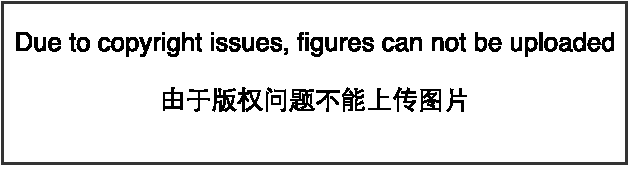
\includegraphics{figure.pdf}}
\else
\centerline{\includegraphics{Chapter14/figures/faces_graph_manifold}}
\fi
\caption{TODO}
\label{fig:chap14_faces_graph_manifold}
\end{figure}

全局坐标系就可以通过优化或求解线性系统获得。
\figref{fig:chap14_tiling-a-manifold}展示了如何通过大量局部线性的类高斯样平铺(或``薄煎饼'',因为高斯块在\gls{tangent_plane}方向是扁平的)得到一个\gls{manifold}。

\begin{figure}[!htb]
\ifOpenSource
\centerline{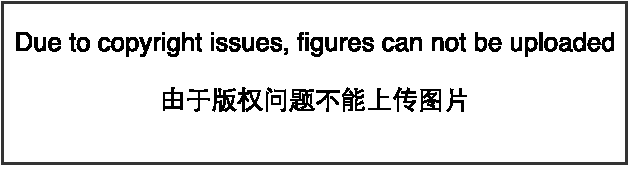
\includegraphics{figure.pdf}}
\else
\centerline{\includegraphics[width=0.8\textwidth]{Chapter14/figures/tiling-a-manifold}}
\fi
\caption{TODO}
\label{fig:chap14_tiling-a-manifold}
\end{figure}

然而,\citet{Bengio+Monperrus-2005}指出了这些局部\gls{nonparametric}方法应用于\gls{manifold_learning}的根本困难:如果\gls{manifold}不是很光滑(它们有许多波峰、波谷和弯曲),我们可能需要非常多的训练样本以覆盖其中的每一个变化,导致没有能力泛化到没见过的变化。
实际上,这些方法只能通过内插,概括相邻实例之间\gls{manifold}的形状。
不幸的是,\glssymbol{AI}问题中涉及的\gls{manifold}可能具有非常复杂的结构,难以仅从局部插值捕获特征。
考虑\figref{fig:chap14_tangent_plane_color}转换所得的\gls{manifold}样例。
如果我们只观察输入向量内的一个坐标$\Vx_i$,当平移图像,我们可以观察到当这个坐标遇到波峰或波谷时,图像的亮度也会经历一个波峰或波谷。
换句话说,底层图像模板亮度的模式复杂性决定执行简单的图像变换所产生的\gls{manifold}的复杂性。
这是采用\gls{distributed_representation}和\gls{DL}来捕获\gls{manifold}结构的动机。

% -- 509 --

\section{\glsentrytext{CAE}}
\label{sec:contractive_autoencoders}
\gls{CAE}\citep{Rifai+al-2011-small,Salah+al-2011-small}在\gls{code}$\Vh = f(\Vx)$的基础上添加了显式的正则项,鼓励$f$的导数尽可能小:
\begin{align}
 \Omega(\Vh) = \lambda \Bigg\| \frac{\partial f(\Vx)}{\partial \Vx} \Bigg\|_F^2 .
\end{align}
惩罚项$\Omega(\Vh)$为平方\ENNAME{Frobenius}范数(元素平方之和),作用于与\gls{encoder}的函数相关\gls{partial_derivatives}的\gls{jacobian}矩阵。


\gls{DAE}和\gls{CAE}之间存在一定联系:\citet{Alain+Bengio-ICLR2013-small}指出在小高斯噪声的限制下,当\gls{reconstruction}函数将$\Vx$映射到$\Vr = g(f(\Vx))$时,\gls{denoising}\gls{reconstruction_error}与\gls{contractive}惩罚项是等价的。
换句话说,\gls{DAE}能抵抗小且有限的输入扰动,而\gls{CAE}使特征提取函数能抵抗极小的输入扰动。

分类任务中,基于\gls{jacobian}的\gls{contractive}惩罚预训练特征函数$f(\Vx)$,将收缩惩罚应用在$f(\Vx)$而不是$g(f(\Vx))$可以产生最好的分类精度。
如\secref{sec:estimating_the_score}所讨论,应用于$f(\Vx)$的\gls{contractive}惩罚与\gls{score_matching}也有紧密的联系。

\firstgls{contractive}源于\glssymbol{CAE}弯曲空间的方式。
具体来说,由于\glssymbol{CAE}是训练成能抵抗输入扰动,鼓励将输入点邻域映射到输出点一更小的邻域。
我们能认为这是将输入的邻域\gls{contractive}到更小的输出邻域。


说得更清楚一点,\glssymbol{CAE}只在局部\gls{contractive}——一个训练样本$\Vx$的所有扰动都映射到$f(\Vx)$的附近。
全局来看,两个不同的点$\Vx$和$\Vx'$会分别被映射到远离原点的两个点$f(\Vx)$和$f(\Vx')$。
$f$扩展到数据\gls{manifold}的中间或远处是合理的(见\figref{fig:chap14_1d_autoencoder_color}中小例子的情况)。
当$\Omega(\Vh)$惩罚应用于\ENNAME{sigmoid}单元时,\gls{contractive}\gls{jacobian}的简单方式是令\ENNAME{sigmoid}趋向饱和的0或1。
这鼓励\glssymbol{CAE}使用\ENNAME{sigmoid}的极值编码输入点,或许可以解释为二进制\gls{code}。
它也保证了\glssymbol{CAE}可以穿过大部分\ENNAME{sigmoid}\gls{hidden_unit}能张成的超立方体,进而扩散其\gls{code}值。

我们可以认为点$\Vx$处的\gls{jacobian}矩阵$\MJ$能将非线性\gls{encoder}近似为线性算子。
这允许我们更形式地使用``\gls{contractive}''这个词。
在线性理论中,当$\MJ\Vx$的范数对于所有单位$\Vx$都小于等于1时,$\MJ$被称为\gls{contractive}的。
换句话说,如果$\MJ$收缩了单位球,他就是\gls{contractive}的。
我们可以认为\glssymbol{CAE}为了鼓励每个局部线性算子具有收缩性,而在每个训练数据点上将\ENNAME{Frobenius}范数作为$f(\Vx)$的局部线性近似的惩罚。


如\secref{sec:learning_manifolds_with_autoencoders}中描述,正则\gls{AE}基于两种相反的推动力学习\gls{manifold}。
在\glssymbol{CAE}的情况下,这两种推动力是\gls{reconstruction_error}和\gls{contractive}惩罚$\Omega(\Vh)$。
单独的\gls{reconstruction_error}鼓励\glssymbol{CAE}学习一个恒等函数。
单独的\gls{contractive}惩罚将鼓励\glssymbol{CAE}学习关于$\Vx$是恒定的特征。
这两种推动力的的折衷产生一个导数$\frac{\partial f(\Vx)}{\partial \Vx}$大多是微小的\gls{AE}。
只有少数\gls{hidden_unit},对应于一小部分输入数据的方向,可能有显著的导数。


\glssymbol{CAE}的目标是学习数据的\gls{manifold}结构。
大的$\MJ\Vx$快速改变$\Vh$的方向$\Vx$很可能是近似\gls{manifold}\gls{tangent_plane}的方向。
\citet{Rifai+al-2011-small,Salah+al-2011-small}的实验显示训练\glssymbol{CAE}会导致$\MJ$中大部分奇异值(幅值)比1小,因此是收缩的。
然而,有些奇异值仍然比1大,因为\gls{reconstruction_error}的惩罚鼓励\glssymbol{CAE}对最大局部变化的方向进行编码。
对应于最大奇异值的方向被解释为\gls{CAE}学到的切方向。
理想情况下,这些切方向应对应于数据的真实变化。
比如,一个应用于图像的\glssymbol{CAE}应该能学到显示图像改变的切向量,如\figref{fig:chap14_tangent_plane_color}图中物体渐渐改变状态。
如\figref{fig:chap14_cifar_cae}所示,实验获得的奇异向量的可视化似乎真的对应于输入图象有意义的变换。

% -- 512 --

\begin{figure}[!htb]
\ifOpenSource
\centerline{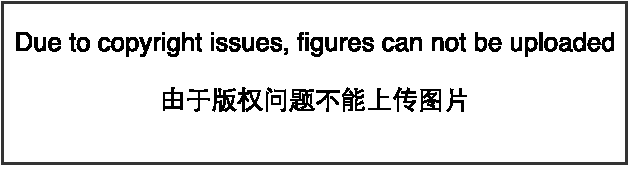
\includegraphics{figure.pdf}}
\else
\centerline{\includegraphics[width=0.8\textwidth]{Chapter14/figures/cifar_cae}}
\fi
\caption{TODO}
\label{fig:chap14_cifar_cae}
\end{figure}

\gls{CAE}\gls{regularization}\gls{criterion}的一个实际问题是,尽管它在单一隐含层的\gls{AE}情况下是容易计算的,但在更深的\gls{AE}情况下会变的难以计算。
根据\citet{Rifai+al-2011-small}的策略,分别训练一系列单层的\gls{AE},并且每个被训练为\gls{reconstruction}前一个\gls{AE}的隐含层。
这些\gls{AE}的组合就组成了一个深度\gls{AE}。
因为每个层分别训练成局部\gls{contractive},深度\gls{AE}自然也是\gls{contractive}的。
这个结果与联合训练深度模型完整架构(带有关于\gls{jacobian}的惩罚项)获得的结果是不同的,但它抓住了许多理想的定性特征。


另一个实际问题是,如果我们不对\gls{decoder}强加一些约束,\gls{contractive}惩罚可能导致无用的结果。
例如,\gls{encoder}将输入乘一个小常数$\epsilon$,\gls{decoder}将\gls{code}除以一个小常数$\epsilon$。
随着$\epsilon$趋向于0,\gls{encoder}会使\gls{contractive}惩罚项$\Omega(\Vh)$趋向于0而学不到任何关于分布的信息。
同时,\gls{decoder}保持完美的\gls{reconstruction}。
\citet{Rifai+al-2011-small}通过绑定$f$和$g$的权重来防止这种情况。
$f$和$g$都是由线性仿射变换后进行逐元素非线性变换的标准\gls{NN}层组成,因此将$g$的权重矩阵设成$f$权重矩阵的转置是很直观的。

% -- 513 --

\section{\glsentrytext{PSD}}
\label{sec:predictive_sparse_decomposition}

\firstall{PSD}是\gls{sparse_coding}和参数化\gls{AE}\citep{koray-psd-08}的混合模型。
参数化\gls{encoder}被训练为能预测迭代推断的输出。
\glssymbol{PSD}被应用与图片和视频中对象识别的\gls{unsupervised}特征学习\citep{Koray-08-small,koray-nips-10-small,Jarrett-ICCV2009-small,farabet-suml-11},在音频中也有所应用\citep{henaff-ismir-11-small}。
这个模型由一个\gls{encoder}$f(\Vx)$和一个\gls{decoder}$g(\Vh)$组成,并且都是参数化的。
在训练过程中,$\Vh$由优化算法控制。
优化过程是最小化
\begin{align}
 \| \Vx - g(\Vh) \| ^2 + \lambda | \Vh |_1 + \gamma \| \Vh - f(\Vx) \|^2.
\end{align}
就像\gls{sparse_coding},训练算法交替地相对$\Vh$和模型的参数最小化上述目标。
相对$\Vh$最小化较快,因为$f(\Vx)$提供$\Vh$的良好初始值以及\gls{loss_function}将$\Vh$约束在$f(\Vx)$附近。
简单的\gls{GD}算法只需10步左右就能获得理想的$\Vh$。


\glssymbol{PSD}所使用的训练程序不是先训练\gls{sparse_coding}模型,然后训练$f(\Vx)$来预测\gls{sparse_coding}的特征。
\glssymbol{PSD}训练过程正则化\gls{decoder},使用$f(\Vx)$可以推断出良好\gls{code}的参数。


\gls{PSD}是\firstgls{learned_approximate_inference}的一个例子。
在\secref{sec:learned_approximate_inference}中,这个话题将会进一步展开。
\chapref{chap:approximate_inference}中展示的工具能让我们了解到,\glssymbol{PSD}能够被解释为最大化模型的对数似然下界来训练有向\gls{sparse_coding}的概率模型。


在\glssymbol{PSD}的实际应用中,迭代优化仅在训练过程中使用。
模型被部署后,参数\gls{encoder}$f$用于计算学习好的特征。
相比于通过\gls{GD}来推断$\Vh$,计算$f$是很容易的。
因为$f$是一个可微带参函数,\glssymbol{PSD}模型可堆叠,并用于初始化其他训练\gls{criterion}的深度网络。

% -- 514 --

\section{\glsentrytext{AE}的应用}
\label{sec:applications_of_autoencoders}

\gls{AE}已成功应用于\gls{dimensionality_reduction}和\gls{information_retrieval}任务。
\gls{dimensionality_reduction}是\gls{representation_learning}和\gls{DL}的第一批应用之一。
它是研究\gls{AE}早期动机之一。
例如, \citet{Hinton-Science2006}训练了一个堆叠\glssymbol{RBM},然后利用它们的权重初始化一个深度\gls{AE}并逐渐变小隐藏层,在30个单元的瓶颈处达到极值。
生成的\gls{code}比30维的\glssymbol{PCA}产生更少的\gls{reconstruction_error},所学的表示更容易定性解释,并能联系基础类别,这些类别表现为分离良好的集群。


低维\gls{representation}可以提高许多任务的性能,例如分类。
小空间的模型消耗更少的内存和运行时间。
据\citet{Salakhutdinov+Hinton2007-small}和\citet{Torralba+Fergus+Weiss-2008}观察,\gls{dimensionality_reduction}的许多形式是跟彼此邻近的例子语义相关的。
映射到低维空间能帮助泛化提示了这个想法。


从\gls{dimensionality_reduction}中比普通任务受益更多的是\gls{information_retrieval},即在数据库中查询类似条目的任务。
此任务从\gls{dimensionality_reduction}获得类似其他任务的一般益处,同时在某些种低维空间中的搜索变得极为高效。
特别的,如果我们训练\gls{dimensionality_reduction}算法来生成一个低维且\emph{二值}的\gls{code},那么我们就可以将所有数据库条目在哈希表映射为二进制编码向量。
这个哈希表允许我们返回具有相同二进制代码的数据库条目作为查询结果进行\gls{information_retrieval}。
我们也可以非常高效地搜索稍有不同条目,只需反转查询编码的各个位。
这种通过\gls{dimensionality_reduction}和二值化的\gls{information_retrieval}方法被称为\firstgls{semantic_hashing}\citep{Salakhutdinov+Hinton2007-small,Salakhutdinov+Geoff-2009},已经被用于文本输入\citep{Salakhutdinov+Hinton2007-small,Salakhutdinov+Geoff-2009}和图像\citep{Torralba+Fergus+Weiss-2008,WeissTF08,KrizhevskyH11}。


通常在最终层上使用\ENNAME{sigmoid}的编码函数来产生\gls{semantic_hashing}的二值\gls{code}。
\ENNAME{sigmoid}单元必须被训练为到达饱和,对所有输入值都接近0或接近1。
能做到这一点的窍门就是训练时在\ENNAME{sigmoid}非线性单元前简单地注入加性噪声。
噪声的大小应该随时间增加。
要对抗这种噪音并且保存尽可能多的信息,网络必须加大输入到\ENNAME{sigmoid}函数的幅度,直到饱和。

% -- 515 --

<BAD>学习哈希函数的思想也在其他几个方向进一步探讨,包括改变损失训练\gls{representation}的想法,这个表示与哈希表中查找附近样本的任务有更直接的联系\citep{Norouzi+Fleet-ICML2011}。
